%------------------------------------------------------------------------------
\chapter{Störkörpermessungen}
\label{sec:stoerkoerpermessung}
%------------------------------------------------------------------------------


%------------------------------------------------------------------------------
\section{Vorbereitung?}
%------------------------------------------------------------------------------

%------------------------------------------------------------------------------
\subsection{Vorbereitung des Resonators}
%------------------------------------------------------------------------------
Bevor mit der Störkörpermessung nach Abschnitt \ref{sec:messmethodik} begonnen werden kann, müssen noch Einstellungen am Resonator erfolgen.
Zum einen wird die Koppelschleife so gedreht, dass eine nahezu kritische Einkopplung ($\kappa \approx 1$) an die $\mathrm{TM}_{010}~\pi$-Mode des Resonators realisiert wird.
Außerdem werden beide Abstimmstempel so eingestellt, dass sich eine symmetrische Feldverteilung im Resonator ausbildet.
Schließlich muss die Beschleunigermode auf ihre Sollfrequenz im Vakuum von $\SI{499.67}{MHz}$ abgestimmt werden.
Dabei gilt es zu beachten, dass die Luft im Hohlraum des Resonators zu einer zusätzlichen Verstimmung führt.
Ist der Resonator durch ein Medium der relativen Permittivität~$\varepsilon_\mathrm{r}$ und Permeabilität~$\mu_\mathrm{r}$ ausgefüllt, so kann die Verstimmung der Resonanzfrequenzen durch
\begin{align}
	\nu_0(\mathrm{Med.}) = \frac{\nu_0(\mathrm{Vak.})}{\sqrt{\varepsilon_\mathrm{r} \mu_\mathrm{r}}}
\end{align}
beschrieben werden \cite{pusch}.
Mit der relativen Permittivität trockener Luft~$\varepsilon_\mathrm{r}^\mathrm{Luft} = \num{1.0005364}$ unter Normalbedingungen \cite[S.\ 1093]{CRC} und der Sollfrequenz im Vakuum folgt die Frequenz der Beschleunigermode
\begin{align}
	\nu_0(\mathrm{Luft}) = \SI{499.54}{MHz}
\end{align}
für den luftgefüllten Resonator.
Da diese Frequenz mit Temperatur und Luftfeuchtigkeit variiert, ist ein exaktes Abstimmen auf diese Frequenz nicht zweckmäßig und es genügt die grobe Einstellung.

%------------------------------------------------------------------------------
\subsection{Bestimmung der Störkörperkonstanten}
%------------------------------------------------------------------------------
Zur Berechnung der Störkörperkonstante~$\alpha_\mathrm{s}$ des kugelförmigen Störkörpers aus PTFE kann Gleichung \eqref{eq:stoerkoerperkonstante} verwendet werden.
Die relative Permittivität von PTFE beträgt im Mittel $\varepsilon_\mathrm{r} = \num{2.1}$ und zeigt eine vernachlässigbare Frequenzabhängigkeit für den in dieser Arbeit untersuchten Frequenzbereich \cite[S.\ 2201]{CRC}.
Außerdem variiert die relative Permittivität mit der Dichte und Kristallinität des Materials, weshalb für den verwendeten Werkstoff $\varepsilon_\mathrm{r} = \num{2.1 +- 0.05}$ angenommen werden muss.
Unter Verwendung der Dimensionen des Störkörpers (vgl.\ \ref{sec:aufbau_messstand}) folgt die Störkörperkonstante
\begin{align}
	\alpha_\mathrm{s} = \SI{2.99 +- 0.11e-17}{\ampere\second\metre\squared\per\volt} \eqcomma
	\label{eq:stoerkoerperkonstante_ptfe}
\end{align}
wobei die zentrische Bohrung bei der Berechnung beachtet wurde.

Bei der Bestimmung der elektrischen Felder gemäß Gleichung \eqref{eq:skm_e_feld_normiert}, wirkt der Fehler der Störkörperkonstanten systematisch auf das resultierende Feld.
Dieser systematische Einfluss muss insbesondere bei der Integration des Feldes über die Störkörperposition (Bestimmung von Beschleunigungsspannung und Shuntimpedanz) gesondert betrachtet werden.
Um diesen Fehler zu verringern, könnte eine direkte Bestimmung der Störkörperkonstanten in einem Referenzresonator durchgeführt werden.
Darauf wurde jedoch in dieser Arbeit verzichtet, da mit einem relativen Fehler von unter $\SI{4}{\percent}$ eine ausreichende Genauigkeit vorliegt.

%------------------------------------------------------------------------------
\subsection{Bestimmung von Resonanzfrequenz und Güte}
\label{sec:resfreq_guete}
%------------------------------------------------------------------------------
Die Bestimmung von Resonanzfrequenz und Güte der Resonatormoden kann anhand des gemessenen Reflexionsspektrums der jeweiligen Resonanz erfolgen.
Dazu wird eine Kurve gemäß Gleichung \eqref{eq:resonanzkurve} nach der Methode der kleinsten Quadrate an das gemessene Spektrum angepasst.
Dies wurde, am Beispiel der $\mathrm{TM}_{010}~\pi$-Beschleunigermode von PETRA-III, in Abbildung \ref{fig:guetefit} dargestellt.
\begin{figure}[htb]
  \centering
  % GNUPLOT: LaTeX picture with Postscript
\begingroup
  \makeatletter
  \providecommand\color[2][]{%
    \GenericError{(gnuplot) \space\space\space\@spaces}{%
      Package color not loaded in conjunction with
      terminal option `colourtext'%
    }{See the gnuplot documentation for explanation.%
    }{Either use 'blacktext' in gnuplot or load the package
      color.sty in LaTeX.}%
    \renewcommand\color[2][]{}%
  }%
  \providecommand\includegraphics[2][]{%
    \GenericError{(gnuplot) \space\space\space\@spaces}{%
      Package graphicx or graphics not loaded%
    }{See the gnuplot documentation for explanation.%
    }{The gnuplot epslatex terminal needs graphicx.sty or graphics.sty.}%
    \renewcommand\includegraphics[2][]{}%
  }%
  \providecommand\rotatebox[2]{#2}%
  \@ifundefined{ifGPcolor}{%
    \newif\ifGPcolor
    \GPcolortrue
  }{}%
  \@ifundefined{ifGPblacktext}{%
    \newif\ifGPblacktext
    \GPblacktexttrue
  }{}%
  % define a \g@addto@macro without @ in the name:
  \let\gplgaddtomacro\g@addto@macro
  % define empty templates for all commands taking text:
  \gdef\gplbacktext{}%
  \gdef\gplfronttext{}%
  \makeatother
  \ifGPblacktext
    % no textcolor at all
    \def\colorrgb#1{}%
    \def\colorgray#1{}%
  \else
    % gray or color?
    \ifGPcolor
      \def\colorrgb#1{\color[rgb]{#1}}%
      \def\colorgray#1{\color[gray]{#1}}%
      \expandafter\def\csname LTw\endcsname{\color{white}}%
      \expandafter\def\csname LTb\endcsname{\color{black}}%
      \expandafter\def\csname LTa\endcsname{\color{black}}%
      \expandafter\def\csname LT0\endcsname{\color[rgb]{1,0,0}}%
      \expandafter\def\csname LT1\endcsname{\color[rgb]{0,1,0}}%
      \expandafter\def\csname LT2\endcsname{\color[rgb]{0,0,1}}%
      \expandafter\def\csname LT3\endcsname{\color[rgb]{1,0,1}}%
      \expandafter\def\csname LT4\endcsname{\color[rgb]{0,1,1}}%
      \expandafter\def\csname LT5\endcsname{\color[rgb]{1,1,0}}%
      \expandafter\def\csname LT6\endcsname{\color[rgb]{0,0,0}}%
      \expandafter\def\csname LT7\endcsname{\color[rgb]{1,0.3,0}}%
      \expandafter\def\csname LT8\endcsname{\color[rgb]{0.5,0.5,0.5}}%
    \else
      % gray
      \def\colorrgb#1{\color{black}}%
      \def\colorgray#1{\color[gray]{#1}}%
      \expandafter\def\csname LTw\endcsname{\color{white}}%
      \expandafter\def\csname LTb\endcsname{\color{black}}%
      \expandafter\def\csname LTa\endcsname{\color{black}}%
      \expandafter\def\csname LT0\endcsname{\color{black}}%
      \expandafter\def\csname LT1\endcsname{\color{black}}%
      \expandafter\def\csname LT2\endcsname{\color{black}}%
      \expandafter\def\csname LT3\endcsname{\color{black}}%
      \expandafter\def\csname LT4\endcsname{\color{black}}%
      \expandafter\def\csname LT5\endcsname{\color{black}}%
      \expandafter\def\csname LT6\endcsname{\color{black}}%
      \expandafter\def\csname LT7\endcsname{\color{black}}%
      \expandafter\def\csname LT8\endcsname{\color{black}}%
    \fi
  \fi
    \setlength{\unitlength}{0.0500bp}%
    \ifx\gptboxheight\undefined%
      \newlength{\gptboxheight}%
      \newlength{\gptboxwidth}%
      \newsavebox{\gptboxtext}%
    \fi%
    \setlength{\fboxrule}{0.5pt}%
    \setlength{\fboxsep}{1pt}%
\begin{picture}(6802.00,4534.00)%
    \gplgaddtomacro\gplbacktext{%
      \csname LTb\endcsname%
      \put(814,704){\makebox(0,0)[r]{\strut{}0{,}0}}%
      \csname LTb\endcsname%
      \put(814,1417){\makebox(0,0)[r]{\strut{}0{,}2}}%
      \csname LTb\endcsname%
      \put(814,2130){\makebox(0,0)[r]{\strut{}0{,}4}}%
      \csname LTb\endcsname%
      \put(814,2843){\makebox(0,0)[r]{\strut{}0{,}6}}%
      \csname LTb\endcsname%
      \put(814,3556){\makebox(0,0)[r]{\strut{}0{,}8}}%
      \csname LTb\endcsname%
      \put(814,4269){\makebox(0,0)[r]{\strut{}1{,}0}}%
      \csname LTb\endcsname%
      \put(1835,484){\makebox(0,0){\strut{}499{,}48}}%
      \csname LTb\endcsname%
      \put(3200,484){\makebox(0,0){\strut{}499{,}50}}%
      \csname LTb\endcsname%
      \put(4565,484){\makebox(0,0){\strut{}499{,}52}}%
      \csname LTb\endcsname%
      \put(5930,484){\makebox(0,0){\strut{}499{,}54}}%
    }%
    \gplgaddtomacro\gplfronttext{%
      \csname LTb\endcsname%
      \put(176,2486){\rotatebox{-270}{\makebox(0,0){\strut{}Reflektionskoeffizient $|\rho|$}}}%
      \put(3675,154){\makebox(0,0){\strut{}Frequenz $\nu$ / \si{MHz}}}%
      \csname LTb\endcsname%
      \put(5418,1097){\makebox(0,0)[r]{\strut{}Messpunkte}}%
      \csname LTb\endcsname%
      \put(5418,877){\makebox(0,0)[r]{\strut{}Anpassung}}%
    }%
    \gplbacktext
    \put(0,0){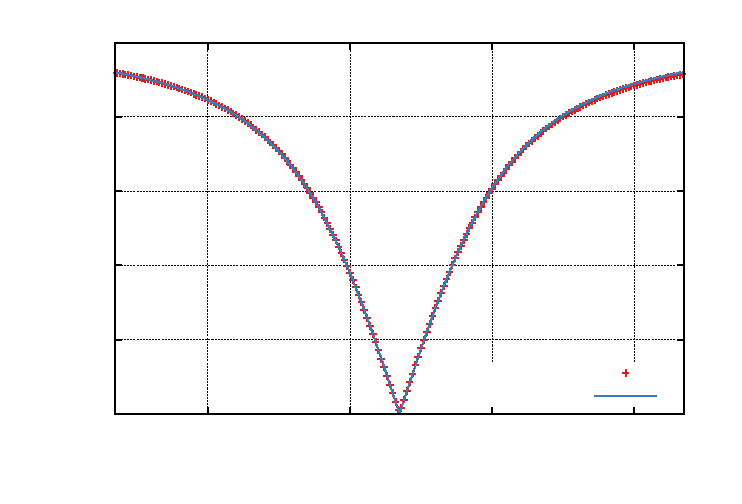
\includegraphics{./plots/guete_fit_pi}}%
    \gplfronttext
  \end{picture}%
\endgroup

  \caption[Anpassung der Resonanzkurve an das Reflexionsspektrum der $\mathrm{TM}_{010}~\pi$-Mode von PETRA-III]{Anpassung der Resonanzkurve~\eqref{eq:resonanzkurve} an ein gemessenes Reflexionsspektrum der $\mathrm{TM}_{010}~\pi$-Mode von PETRA-III. Aus Gründen der Übersicht wurde nur jeder 10.\ Messpunkt des VNA aufgetragen. Die Anpassung liefert die Resonanzfrequenz~$\nu_0 = \SI{499.537 +- 0.001}{MHz}$ \todo{$\Delta$}, Güte~$Q_0 = \num{29560 +- 20}$ und den Koppelfaktor~$\kappa = \num{1.013 +- 0.001}$.}
  \label{fig:guetefit}
\end{figure}
Um eine bessere Abschätzung der Fehler zu erlauben, wurden zu jeder Resonatormode mehrere Reflexionsspektren aufgenommen und an jedes Spektrum eine Anpassung durchgeführt.
Die resultierenden Ergebnisse folgen aus der Bildung des Mittelwerts der angepassten Parameter.

\todo{Frequenzgenauigkeit, Leitfähigkeit $\Delta Q_0 \approx \SI{1}{\percent}$}


\section{Vermessung der TM010 Beschleunigermode}
Berechnung des elektrischen Feldes\\
Berechnung der charakteristischen Größen des Resonators: Beschleunigungsspannung, Shuntimpedanz und Laufzeitfaktor

Alle anderen Moden (5/6, 1/2, 1/6) haben verschwindende Felder in der zentralen Zelle und können damit nicht gekoppelt werden.

Längenmessung vom Flansch erklären.


\section{Vermessung von Moden höherer Ordnung (PETRA-III)}
